% Options for packages loaded elsewhere
\PassOptionsToPackage{unicode}{hyperref}
\PassOptionsToPackage{hyphens}{url}
%
\documentclass[
]{article}
\usepackage{amsmath,amssymb}
\usepackage{iftex}
\ifPDFTeX
  \usepackage[T1]{fontenc}
  \usepackage[utf8]{inputenc}
  \usepackage{textcomp} % provide euro and other symbols
\else % if luatex or xetex
  \usepackage{unicode-math} % this also loads fontspec
  \defaultfontfeatures{Scale=MatchLowercase}
  \defaultfontfeatures[\rmfamily]{Ligatures=TeX,Scale=1}
\fi
\usepackage{lmodern}
\ifPDFTeX\else
  % xetex/luatex font selection
\fi
% Use upquote if available, for straight quotes in verbatim environments
\IfFileExists{upquote.sty}{\usepackage{upquote}}{}
\IfFileExists{microtype.sty}{% use microtype if available
  \usepackage[]{microtype}
  \UseMicrotypeSet[protrusion]{basicmath} % disable protrusion for tt fonts
}{}
\makeatletter
\@ifundefined{KOMAClassName}{% if non-KOMA class
  \IfFileExists{parskip.sty}{%
    \usepackage{parskip}
  }{% else
    \setlength{\parindent}{0pt}
    \setlength{\parskip}{6pt plus 2pt minus 1pt}}
}{% if KOMA class
  \KOMAoptions{parskip=half}}
\makeatother
\usepackage{xcolor}
\usepackage[margin=1in]{geometry}
\usepackage{longtable,booktabs,array}
\usepackage{calc} % for calculating minipage widths
% Correct order of tables after \paragraph or \subparagraph
\usepackage{etoolbox}
\makeatletter
\patchcmd\longtable{\par}{\if@noskipsec\mbox{}\fi\par}{}{}
\makeatother
% Allow footnotes in longtable head/foot
\IfFileExists{footnotehyper.sty}{\usepackage{footnotehyper}}{\usepackage{footnote}}
\makesavenoteenv{longtable}
\usepackage{graphicx}
\makeatletter
\def\maxwidth{\ifdim\Gin@nat@width>\linewidth\linewidth\else\Gin@nat@width\fi}
\def\maxheight{\ifdim\Gin@nat@height>\textheight\textheight\else\Gin@nat@height\fi}
\makeatother
% Scale images if necessary, so that they will not overflow the page
% margins by default, and it is still possible to overwrite the defaults
% using explicit options in \includegraphics[width, height, ...]{}
\setkeys{Gin}{width=\maxwidth,height=\maxheight,keepaspectratio}
% Set default figure placement to htbp
\makeatletter
\def\fps@figure{htbp}
\makeatother
\setlength{\emergencystretch}{3em} % prevent overfull lines
\providecommand{\tightlist}{%
  \setlength{\itemsep}{0pt}\setlength{\parskip}{0pt}}
\setcounter{secnumdepth}{5}
\usepackage{float}
\usepackage{booktabs}
\usepackage{longtable}
\usepackage{array}
\usepackage{multirow}
\usepackage{wrapfig}
\usepackage{colortbl}
\usepackage{pdflscape}
\usepackage{tabu}
\usepackage{threeparttable}
\usepackage{threeparttablex}
\usepackage[normalem]{ulem}
\usepackage{makecell}
\usepackage{xcolor}
\ifLuaTeX
  \usepackage{selnolig}  % disable illegal ligatures
\fi
\usepackage[]{natbib}
\bibliographystyle{plainnat}
\usepackage{bookmark}
\IfFileExists{xurl.sty}{\usepackage{xurl}}{} % add URL line breaks if available
\urlstyle{same}
\hypersetup{
  pdftitle={Towards combined epidemiological and economic dynamical systems},
  hidelinks,
  pdfcreator={LaTeX via pandoc}}

\title{Towards combined epidemiological and economic dynamical systems}
\author{}
\date{\vspace{-2.5em}}

\begin{document}
\maketitle

This document describes some combined epi-econ models, starting with DAEDALUS, and then moving onto SFC-epi models.

Code examples are taken and adapted from \url{https://github.com/marcoverpas/Italy-SFC-Model} and \url{https://github.com/marcoverpas/Six_lectures_on_sfc_models}.

\section{DAEDALUS}\label{daedalus}

Originally designed of for the UK \citep{Haw2020} and since applied to Indonesia \citep{Johnson2023}. The econ model is static. The industrial sectors of the economy are used to stratify the population in the epi model, in which there are contacts related to sector of work and consumption.

In response to an outbreak, closures are mandated, resulting in operations in each sector reducing to some percentage. In the model, GVA reduces to the same percentage, and so does attendance of places of work and consumption, which scales contacts made and subsequently disease transmission.

The population is static: it does not grow, and no one changes sector of work. The non-working group remains non-working. The workforce in place includes a fraction who work from home and therefore contribute to GVA but not infections from workplace interactions.

See \url{https://github.com/robj411/p2_drivers} for a recent presentation.

\begin{figure}

\includegraphics[width=0.7\linewidth]{README_files/figure-latex/dae-1} \caption{Daedalus model. Mandated closures reduce both infections and workforce in place.}\label{fig:dae}
\end{figure}

\section{SFC-epi}\label{sfc-epi}

We will use an SFC model in place of GVA by sector. The SFC model is dynamic in time, meaning impacts can accumulate, and is demand driven, meaning we can model autonomous behaviour changes that will have impacts on both the economy and the epidemic.

At present we compute the ``propensity to consume/work'' which scales the contacts in the epi model and feeds into the econ model. It might be better to precompute the counterfactual (without epidemic) consumption and labour, and:

\begin{enumerate}
\def\labelenumi{\arabic{enumi}.}
\tightlist
\item
  compute scaled parameters using epi variable(s) and response function;
\item
  solve econ model to get consumption and labour;
\item
  scale contacts with the same ratio as consumption and labour have to the no-epidemic counterfactual at the same time point
\end{enumerate}

NB: the model assumes an impact on the general population (i.e.~both susceptibles and infectious change their behaviour). Lack of consumption and work from people who are already sick \emph{because} they are sick is not modelled. This could be included explicitly by e.g.~setting the proportion of non-diseased people as the upper bound to propensities.

\begin{figure}
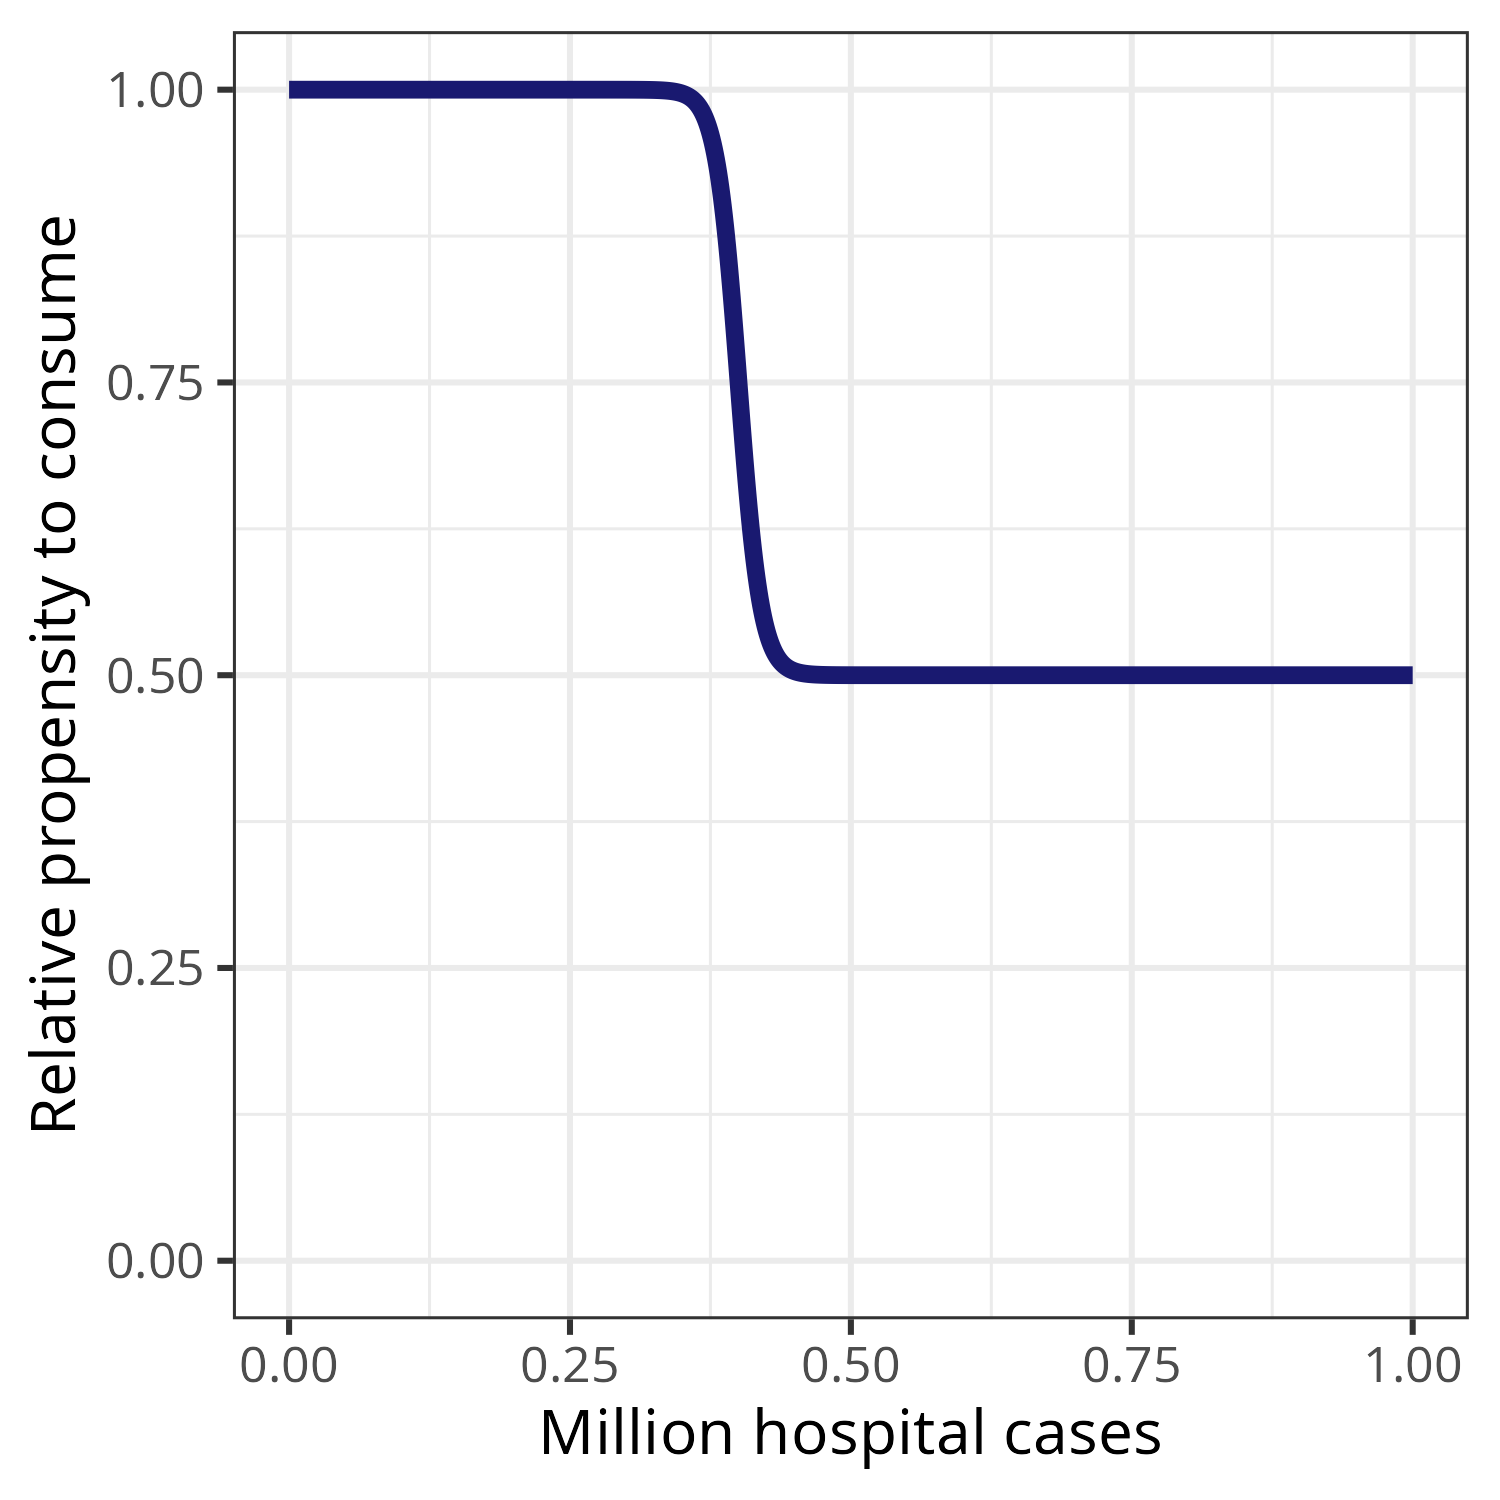
\includegraphics[width=0.5\linewidth]{figures/response} \caption{Dose--response function: extent of behaviour change as a function of an epidemiological variable such as number of hospital cases.}\label{fig:unnamed-chunk-1}
\end{figure}

\subsection{Consumption}\label{consumption}

\begin{figure}

\includegraphics[width=0.7\linewidth]{README_files/figure-latex/consumption-1} \caption{Epi variables reduce propensity to consume, which reduces consumption, and therefore GVA and new infections.}\label{fig:consumption}
\end{figure}

The first step is to model consumption as a function of the epidemic, e.g.~the number of cases, hospitalisations or deaths. The epidemic variable modifies the ``propensity to consume'' parameters (often labelled \(\alpha\)). We scale propensity to consume and exposure-related activities by the same amount.

\begin{figure}
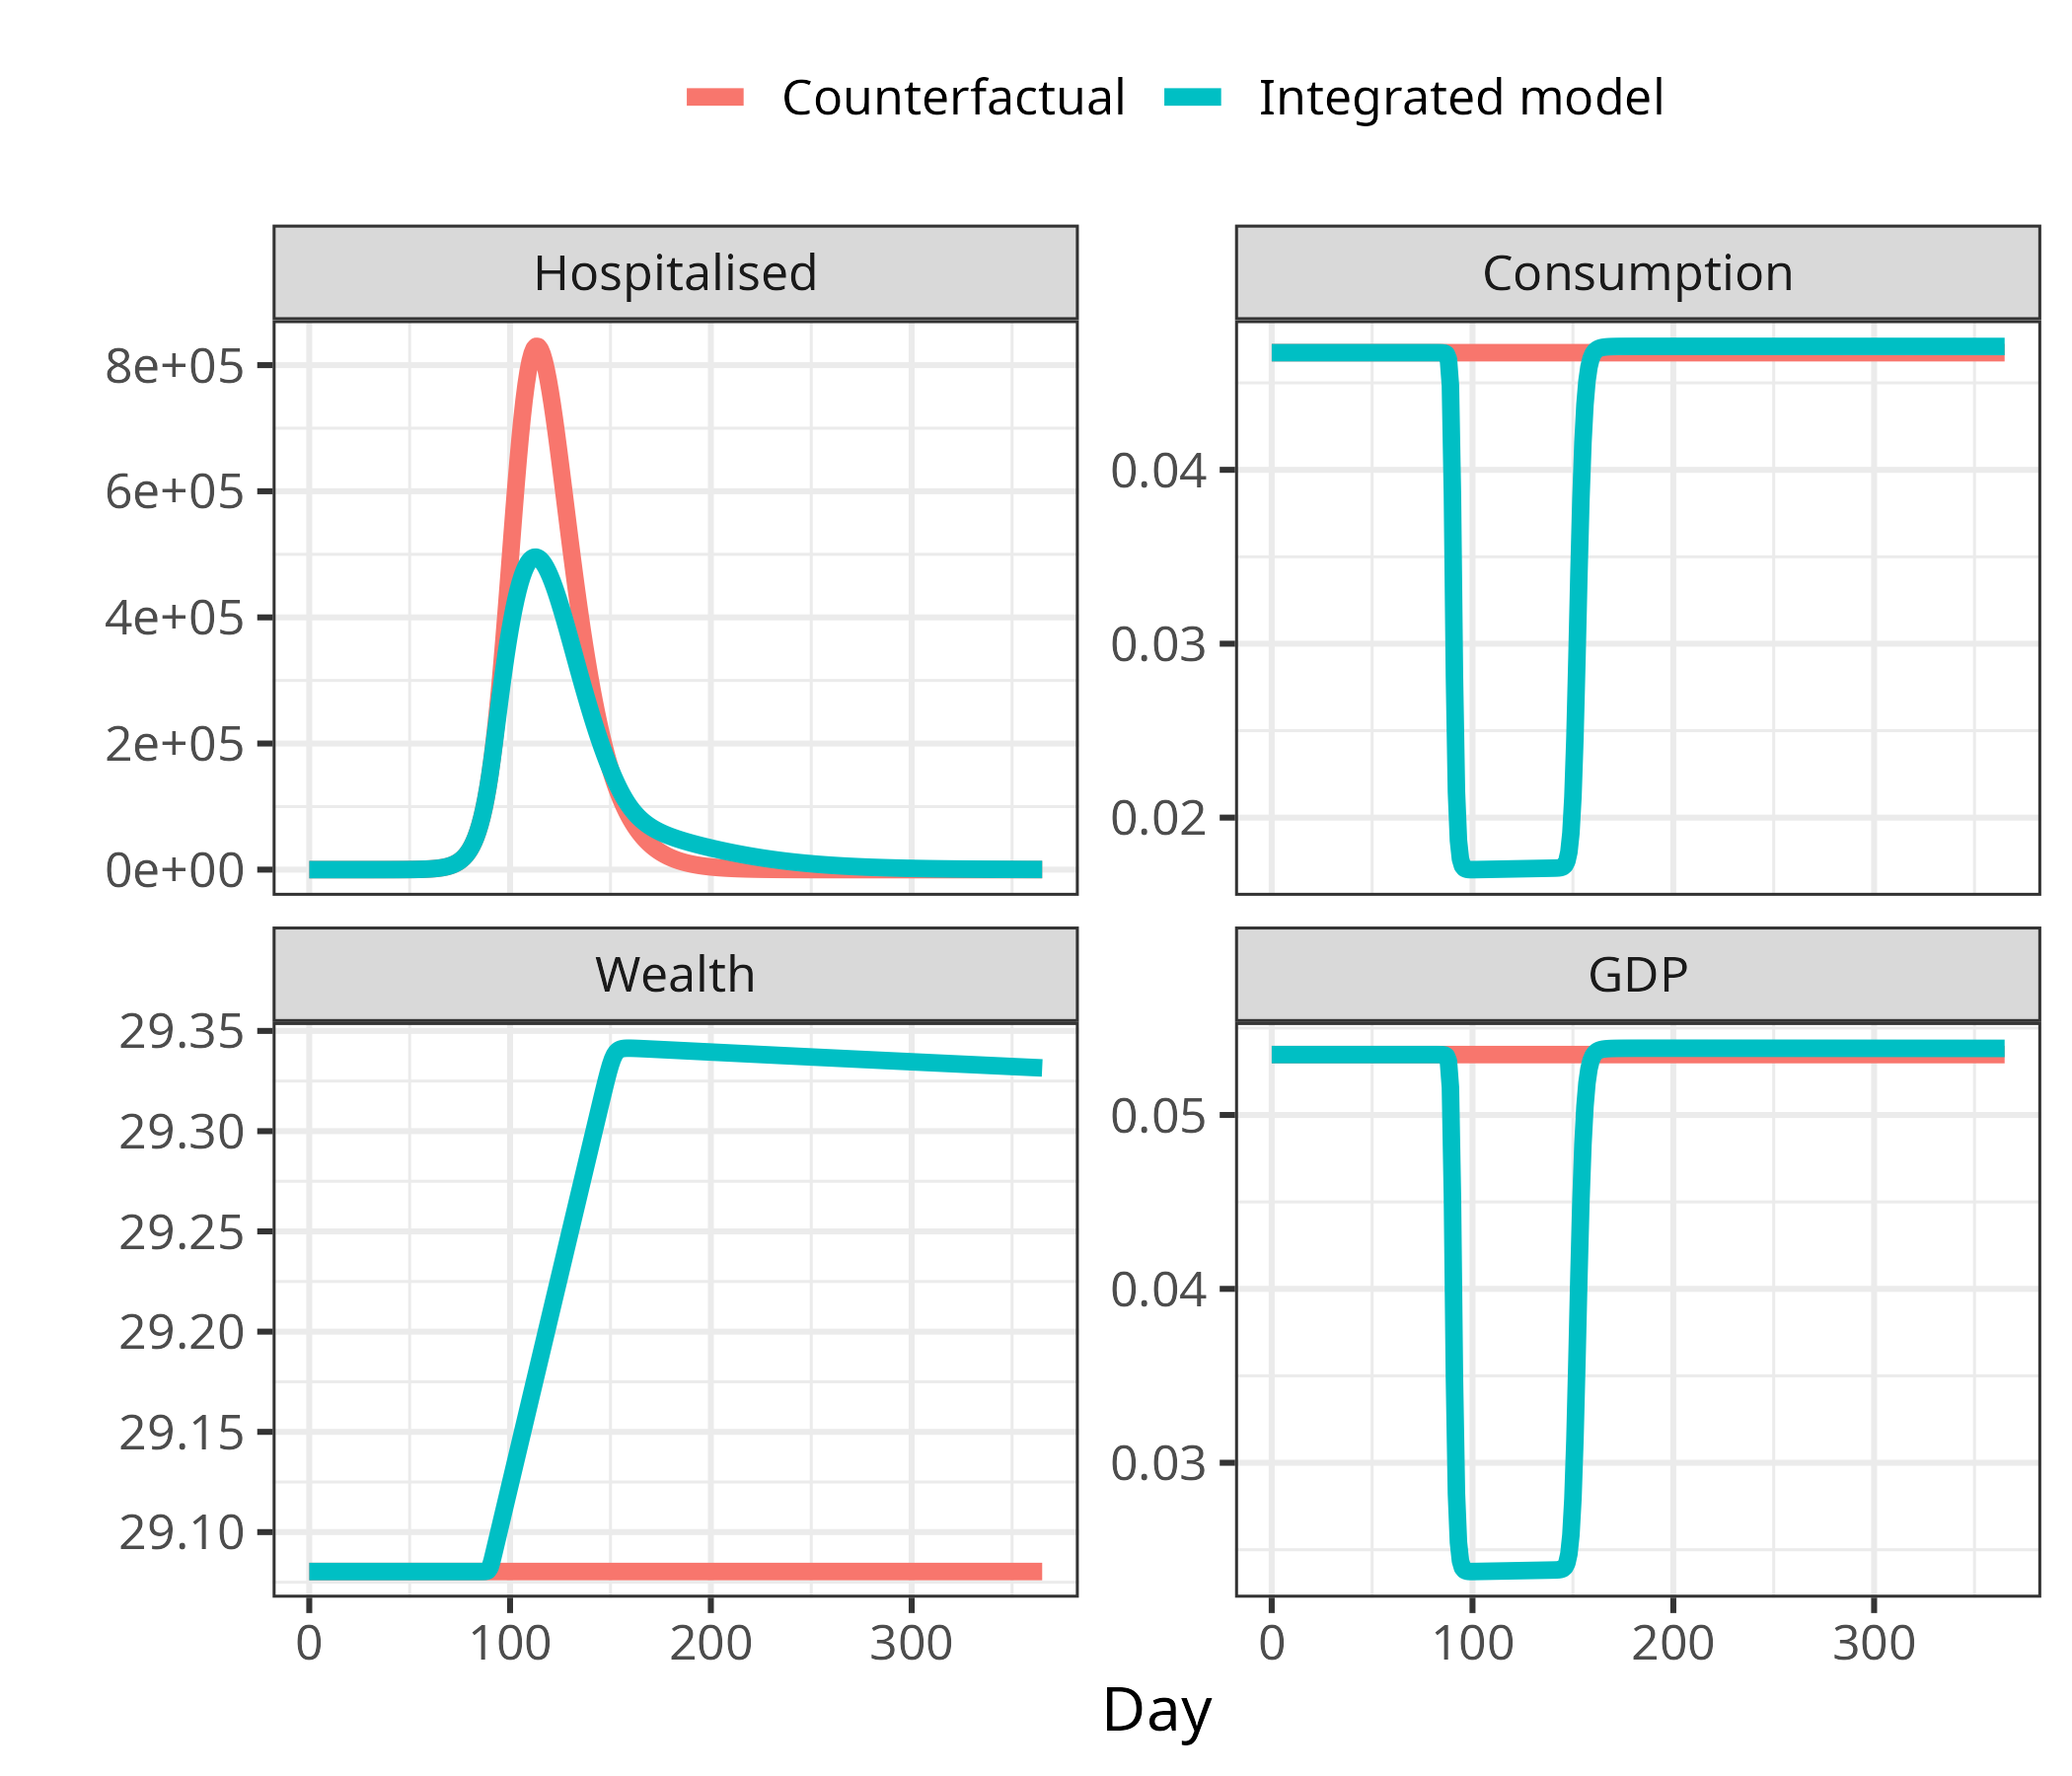
\includegraphics[width=0.8\linewidth]{figures/pc_plot} \caption{Results for PC model with consumption reduction alongside counterfactual epi and econ curves without integration.}\label{fig:unnamed-chunk-2}
\end{figure}

\subsection{Labour supply}\label{labour-supply}

\begin{figure}

\includegraphics[width=0.7\linewidth]{README_files/figure-latex/labour-1} \caption{Epi variables reduce propensity to work and to consume, which reduces consumption and labour supply, and therefore GVA and new infections.}\label{fig:labour}
\end{figure}

Next, we model reduction in propensity to work in the same way.

However, this should ultimately depend also on the need for income, meaning that (a) lower income people are more likely to work, (b) people are more likely to work as time goes on and they've spent some months with less income, and (c) we can later mitigate these effects to some extent with government transfers.

This version of the model (with spontaneous consumption and labour change) can be used to model an unmitigated epidemic: that is, an epidemic where there are no government interventions, but the population can choose infection-avoiding behaviours, which will dampen both the epidemic and the economy. This is an important gap in current epi modelling. We usually assume either no behaviour change, so that unmitigated epidemics have huge death tolls (e.g.~UK COVID projection), or that uncosted (free) population behaviour change will curb the excesses of the epidemic (CEPI work).

\subsection{Mandated closures}\label{mandated-closures}

\begin{figure}

\includegraphics[width=0.7\linewidth]{README_files/figure-latex/mandate-1} \caption{Epi variables reduce propensity to work and to consume, which reduces consumption and labour supply, and therefore GVA and new infections. Mandated closures reduce consumption and propensity to work.}\label{fig:mandate}
\end{figure}

Next we want to introduce the ability for the government to mandate closures. This might be modelled as e.g.~a maximum labour demand, expressed as a percentage of counterfactual labour demand.

Propose a worked example, such as ``how would we model a mandate that the hospitality sector closes?''

\subsection{Government transfers}\label{government-transfers}

\begin{figure}

\includegraphics[width=0.7\linewidth]{README_files/figure-latex/transfers-1} \caption{Epi variables reduce propensity to work and to consume, which reduces consumption and labour supply, and therefore GVA and new infections. Mandated closures reduce consumption and propensity to work. Government transfers increase consumption and reduce propensity to work.}\label{fig:transfers}
\end{figure}

We should introduce government transfers to demonstrate that mandated closures are only sustainable for as long as the population is supported to forego income in order to stop the spread of infection.

\subsection{Other (important) things to consider}\label{other-important-things-to-consider}

\begin{itemize}
\tightlist
\item
  international trade, esp.~tourism
\item
  structural changes over time?
\item
  move to online consumption
\end{itemize}

\section{Epidemic model}\label{epidemic-model}

I propose that, for the epidemic model, we remain as consistent as possible with DAEDALUS:

\begin{itemize}
\tightlist
\item
  four age groups (pre-school age, school-age children, working age, retirement age)
\item
  working-age people stratified by something: definitely working/not working, potentially something sector, occupation or SES related
\item
  seven disease states (S, E, I (symptomatic/asymptomatic), R, H, D)
\item
  no vaccination or waning, for simplicity
\item
  leave school closures out for now, for simplicity
\item
  outputs from the econ model parametrise the function \(k_{j}^{1}\)
\end{itemize}

\subsection{Ordinary differential equations}\label{ordinary-differential-equations}

\begin{align}
\frac{dS_{j}}{dt} & = - k_{j}^{1}(t)S_{j}  \\
\frac{dE_{j}}{dt} & = k_{j}^{1}(t)S_{j} - (k^2+k^4)E_{j} \\
\frac{dI_{j}^a}{dt} & = k^2E_{j} - k^3I_{j}^a \\
\frac{dI_{j}^s}{dt} & = k^4E_{j} - (k_{j}^{5}+k_{j}^{6})I_{j}^s \\
\frac{dR_{j}}{dt} & = k^3I_{j}^a + k_{j}^{5}I_{j}^s + k_{j}^{7}(t) H_{j}\\
\frac{dH_{j}}{dt} & = k_{j}^{6}I_{j}^s - (k_{j}^{7}(t) + k_{j}^{8}(t)) H_{j} \\
\frac{dD_{j}}{dt} & =  k_{j}^{8}(t) H_{j}
\end{align}

\subsection{Disease state transitions}\label{disease-state-transitions}

\begin{figure}

\includegraphics[width=0.5\linewidth]{README_files/figure-latex/statetransitions-1} \caption{Disease state transitions. $S$: susceptible. $E$: exposed. $I^{a}$: asymptomatic infectious. $I^{s}$: symptomatic infectious. $H$: in need of hospitalisation. $R$: recovered. $D$: died. $j$: stratum.}\label{fig:statetransitions}
\end{figure}

\renewcommand\refname{References}
  \bibliography{DAEDALUS.bib}

\end{document}
